\section{Versione mobile}\label{mobile}

TicketOne non ha una versione mobile particolarmente curata, ma questa è solamente un adattamento del sito desktop che è stato fatto seguendo le regole di \textit{responsiveness} e permettendo un adattamento ai vari browser e alle varie risoluzioni dello schermo.
\par La homepage di TicketOne in versione mobile (Fig.~\ref{mobile1}) si presenta in maniera molto simile alla controparte desktop: l'header contiene ancora la barra di ricerca e un paio di pulsanti che corrispondono ad ``\textit{Eventi}'' e ``\textit{Località}'', visibili in Fig.~\ref{homepage}.
Rimane presente anche il carosello degli eventi principali, ovviamente riadattato alla dimensione ridotta dello schermo e il \textit{prospect ratio} differente rispetto al desktop.
Restano intatte le sezioni con gli eventi divisi per categoria.
\par Alcune informazioni sono state tolte, come lo slogan del sito, oppure spostate in fondo alla pagina come la possibilità di poter scegliere la lingua.

\begin{figure}[H]
	\centering
	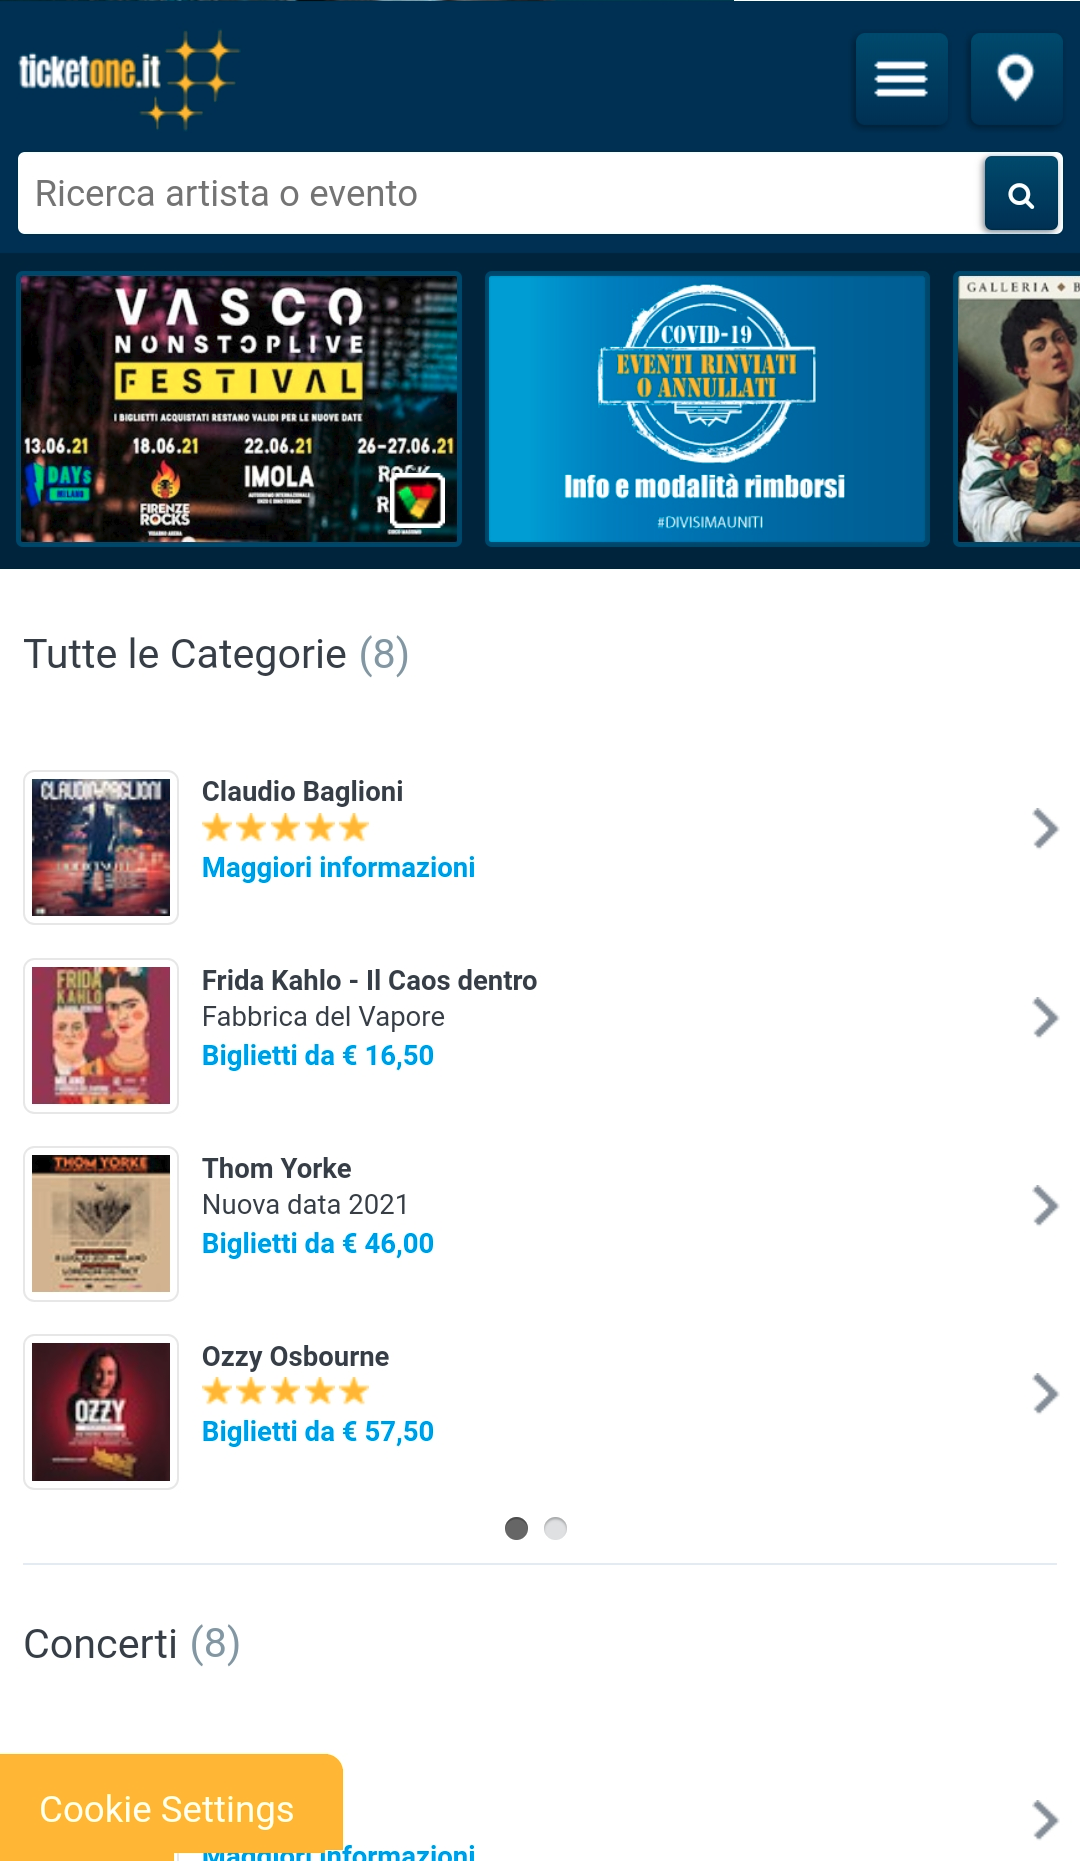
\includegraphics[width=7cm]{img/mobile_1.png}
	\caption{Homepage di TicketOne versione mobile}
	\label{mobile1}
\end{figure}

\subsection{Ricerca in versione mobile}

	Come per il desktop, la barra di ricerca mostra i suggerimenti in maniera dinamica suddividendoli per la categoria a cui appartengono i risultati (Fig.~\ref{mobile2}).
	
	\begin{figure}[H]
		\centering
		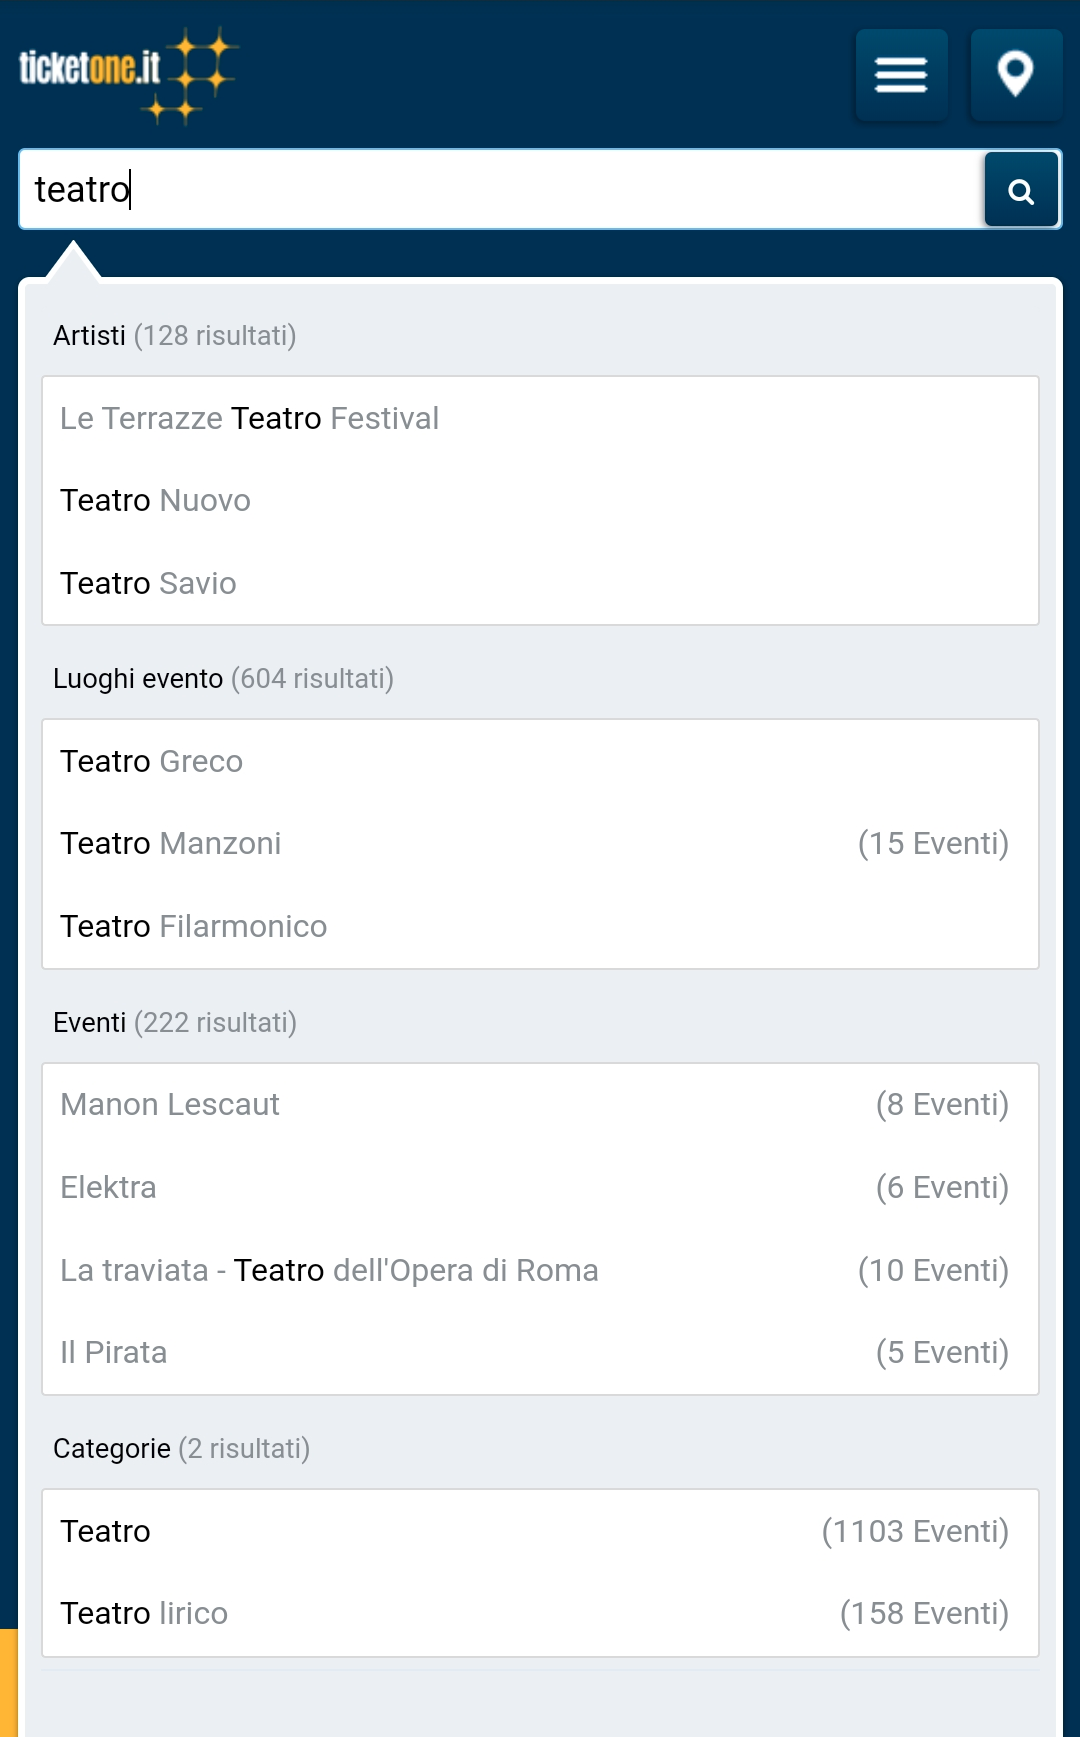
\includegraphics[width=7.5cm]{img/mobile_2.png}
		\caption{Suggerimenti di ricerca in versione mobile}
		\label{mobile2}
	\end{figure}
	
	Nella pagina in cui vengono presentati i risultati di ricerca, per risparmiare spazio, il menu che nella versione desktop è nella colonna di sinistra (Fig.~\ref{ricerca2}) e che rappresenta le categorie in cui figurano i risultati, viene trasformato in un menu che appare o scompare premendo un pulsante sotto all'header (Fig.~\ref{mobile3}).
	
	\begin{figure}[H]
		\centering
		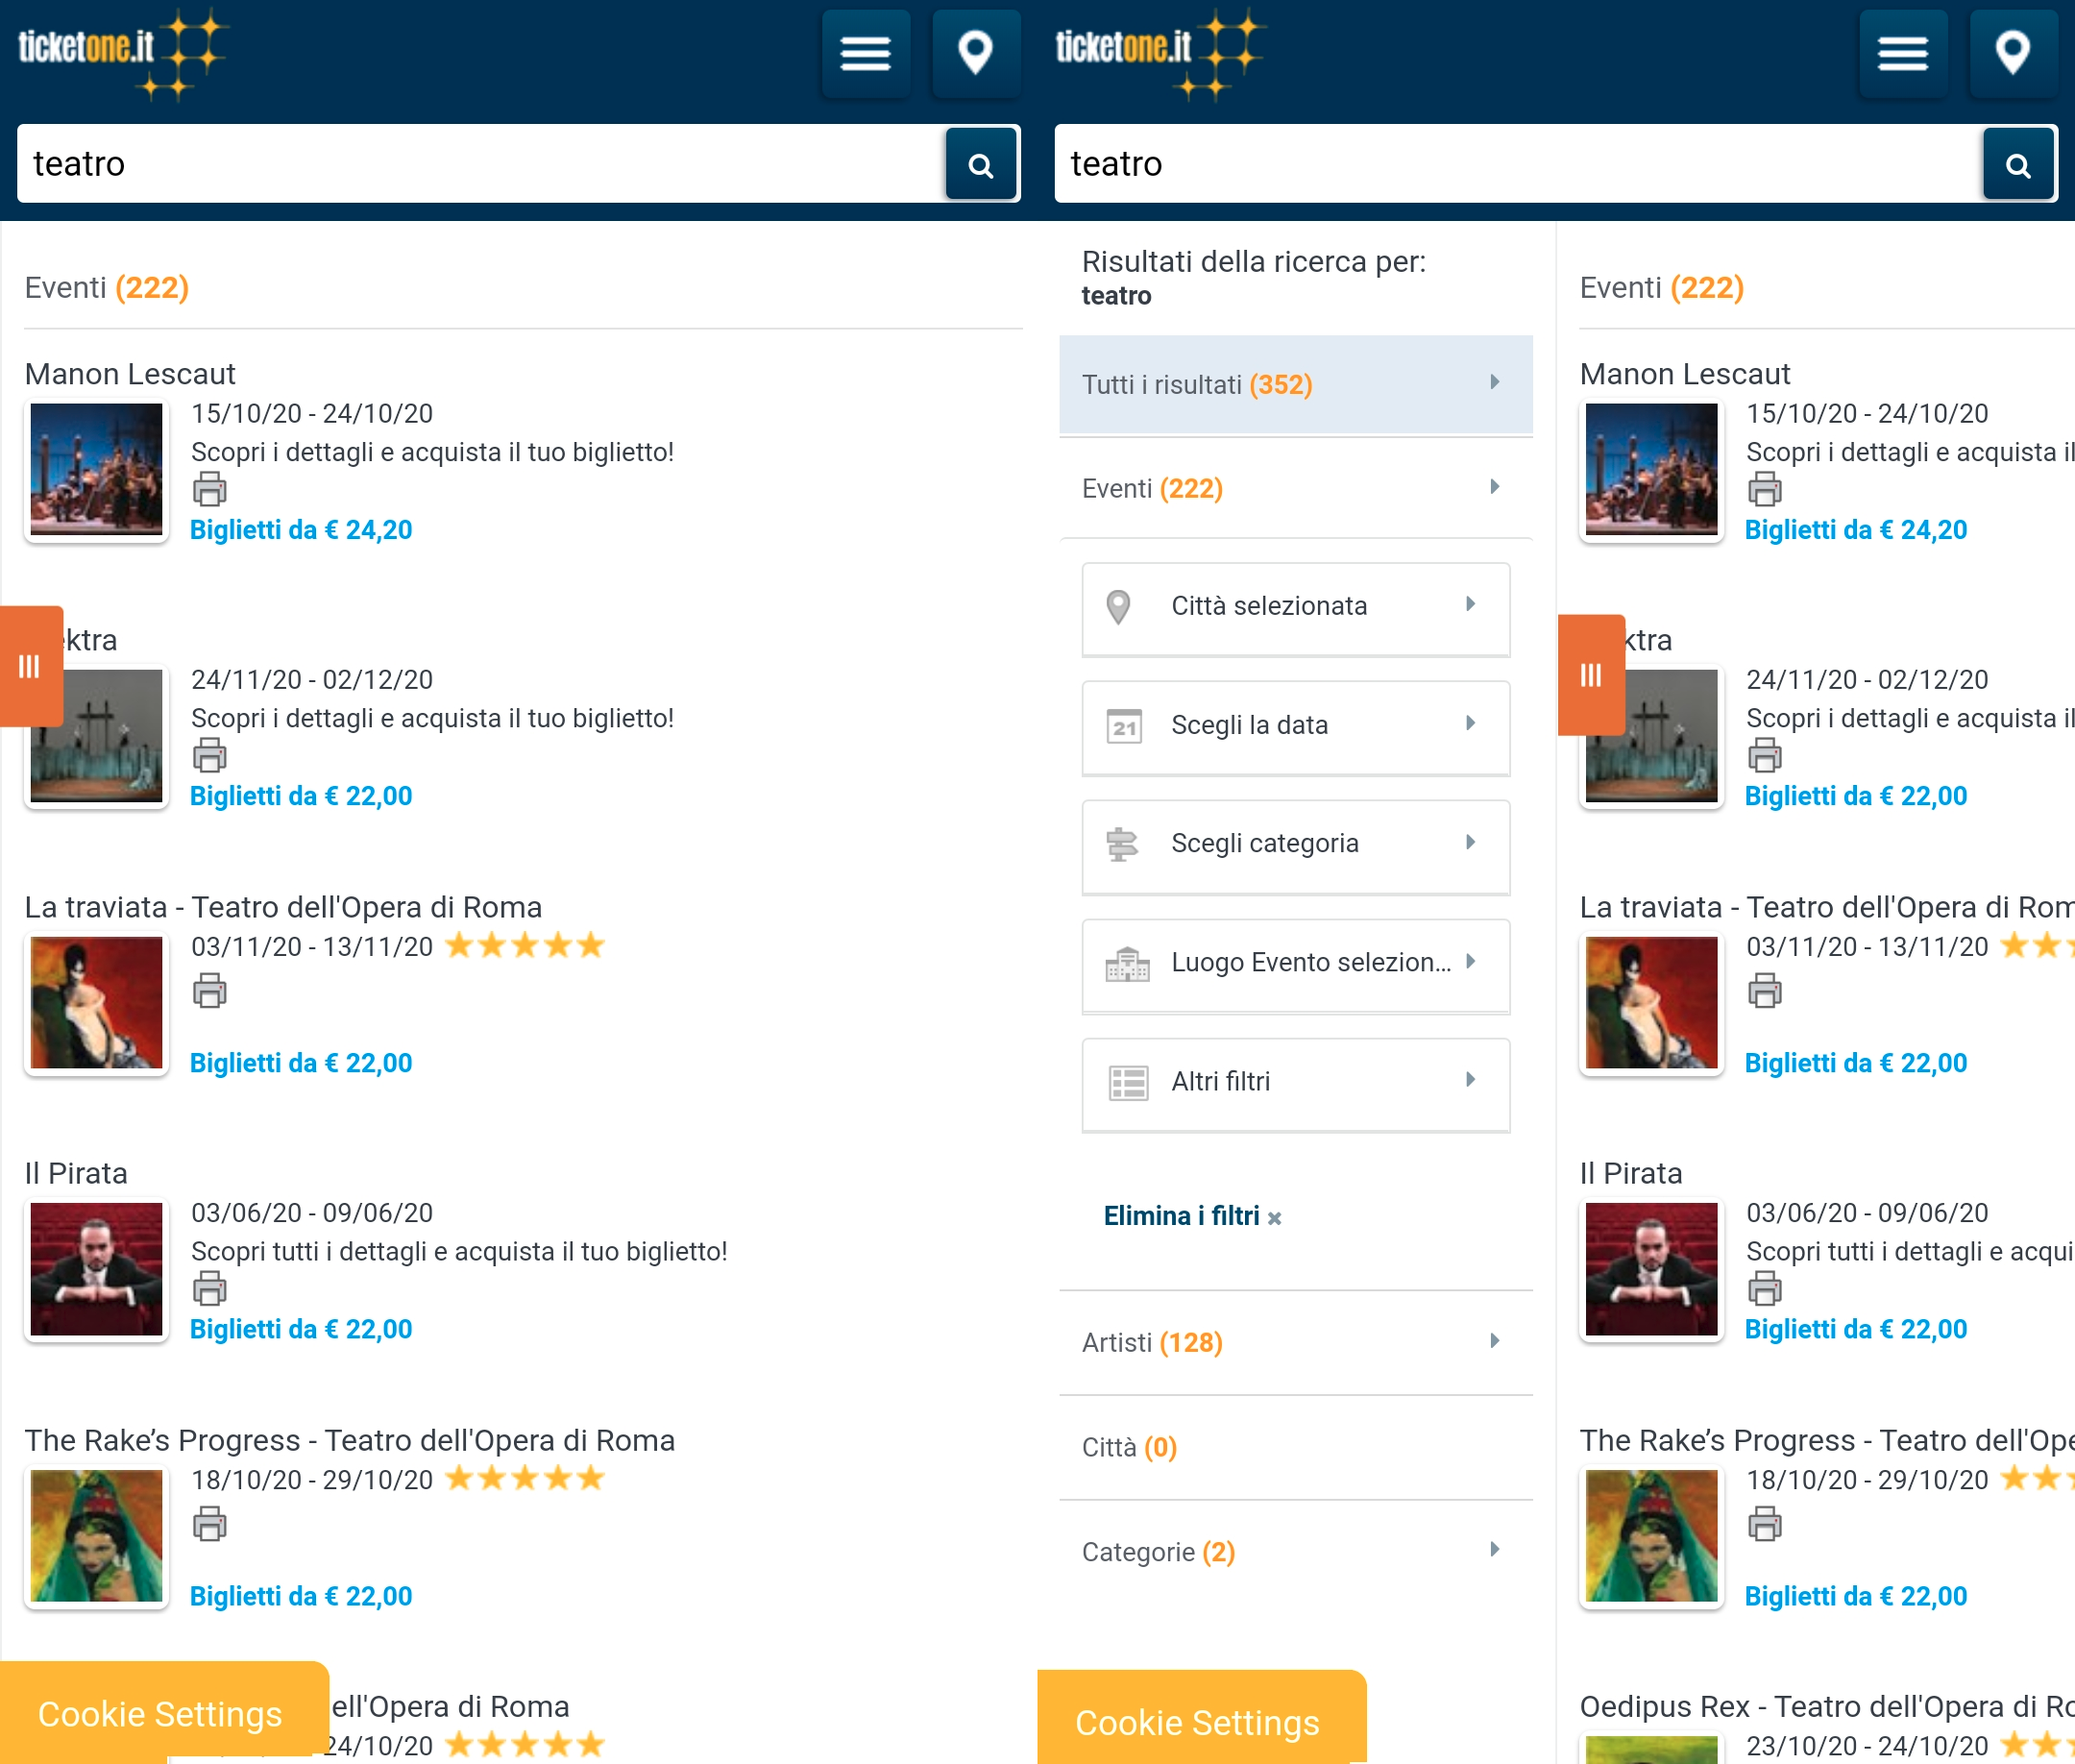
\includegraphics[width=\textwidth]{img/mobile_3.png}
		\caption{Risultati di ricerca in versione mobile}
		\label{mobile3}
	\end{figure}

\subsection{Applicazione}

	Oltre alla versione mobile del sito è presente un'applicazione ufficiale di TicketOne (Fig.~\ref{mobile4}) che permette di effettuare le stesse operazioni della piattaforma desktop (e mobile).
	\'E possibile scaricare questa applicazione dagli store ufficiali di Google ed Apple.
	\par Questa è stata fatta per permettere all'utente di effettuare ricerche in maniera più efficiente data la dimensione dello schermo e tenendo conto che l'interfaccia non è più il mouse ma il \textit{dito}, che quindi ha una superficie maggiore.
	Complessivamente l'applicazione ufficiale di TicketOne offre una migliore \textit{User Expercience} (o \textit{UX}) sulle piattaforme mobili rispetto all'utilizzo del sito in versione ridotta.
	
	\begin{figure}[H]
		\centering
		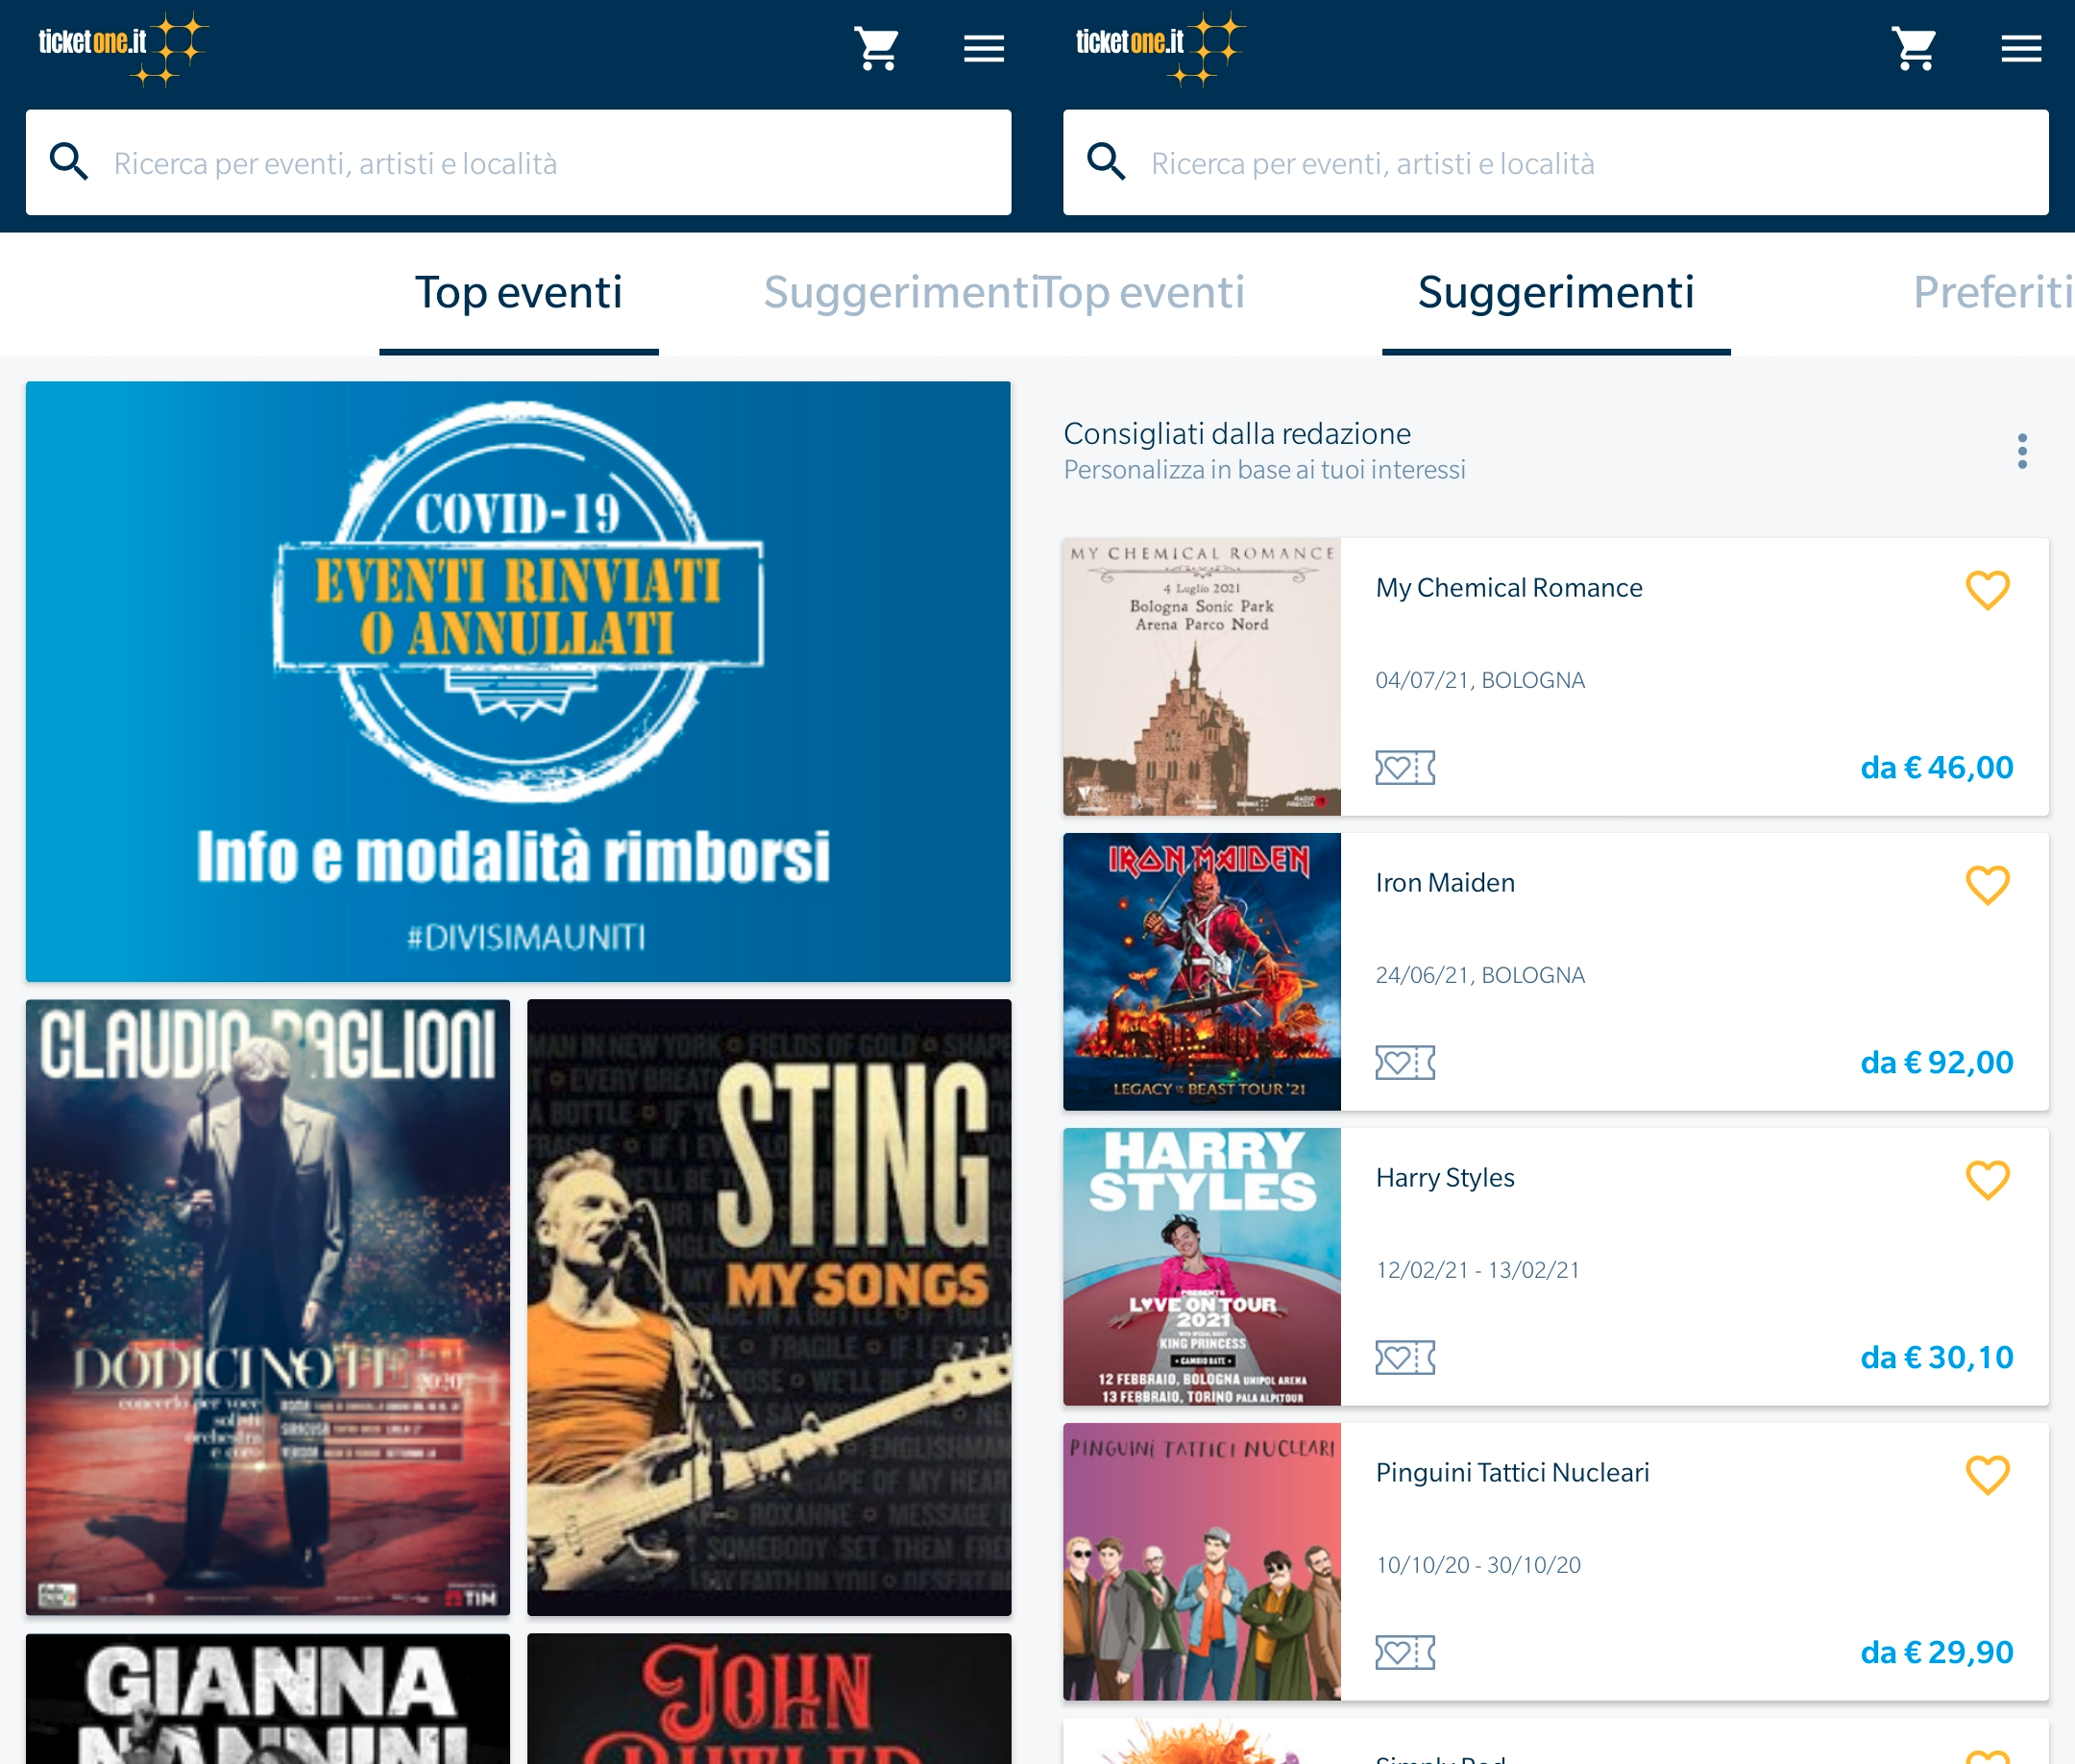
\includegraphics[width=\textwidth]{img/mobile_4.png}
		\caption{Interfaccia dell'applicazione mobile}
		\label{mobile4}
	\end{figure}